\section{Evaluation} \label{sec:vibvoice_evaluation}

\subsection{Experiment Setup} \label{sec:vibvoice_experiment}
We use EarSense introduced in Section. \ref{sec:vibvoice_EarSense} to collect audio and acceleration signals simultaneously\footnote{The experiments that involve human subjects have been approved by the IRB of the authors' institution (CUHK-SBRE-21-0570).}. The volunteers are asked to wear EarSense and speak in a meeting room with the size of $10~\text{m}^2$. The reading material is selected from daily English conversations \citep{Everyday75:online}. Each volunteer reads the material for 30 seconds and repeats it 20 times, generating ten minutes of data. For data augmentation, we recruit eight volunteers to generate a pool of Bone Conduction Functions and use it to augment 100 hours of data from LibriSpeech \citep{panayotov2015librispeech}. 
In addition, we recruit another 15 volunteers for training and testing. For each experiment, we adopt the leave-one-out validation, i.e., training the model for each user with the dataset except that user. The volume of our collected speech is between 60dB to 70dB, which is the same as regular conversations \citep{WhatNois20:online}.
To test VibVoice's robustness to diverse noises, we use three categories of noises with balanced possibility, including environmental noises (50 classes) \citep{piczak2015dataset}, competing speakers from another subset of LibriSpeech \citep{panayotov2015librispeech}, and 20 songs with languages of English, Mandarin, and Japanese. We apply a random room impulse response from dataset \citep{ko2017study}, containing point-source noises, real isotropic noises, and simulated the noises of 600 rooms.
We implement VibVoice using PyTorch and train it on a PC with an Intel i9-12900K CPU and two Nvidia RTX 3090 GPUs. 
The model is trained with a step learning rate scheduler with a learning rate of 0.001 and an Adam optimizer. The epoch number is 30.
The length of the STFT window and the overlap for the audio are 640 and 320, while 64 and 32 are for the acceleration. We open-source the implementation and data in \citep{dataset}.

\subsection{Baseline}
We deploy two baselines, i.e., FullSubNet (FSN) \citep{hao2021fullsubnet} and SEANet (SN) \citep{tagliasacchi2020seanet}.
FSN and SN are two state-of-the-art speech enhancement approaches using audio-only and audio-acceleration inputs, respectively.
We train SN using our dataset since the one used in its paper is not available to the public. Specifically, we train SN using acceleration data with a sample rate of 1.6kHz to ensure it is the same as VibVoice. Note that SN indicates that it supports acceleration data with a wide range of sample rates.

\subsection{Evaluation Metric}\label{metric}
We use three evaluation metrics, i.e., Perceptual Evaluation of Speech Quality (PESQ), Signal Noise Ratio (SNR), and Log-Spectral Distance (LSD), which are described as follows:

%\vspace{0.5em}
\noindent\textit{Perceptual Evaluation of Speech Quality (PESQ)}
is a popular test standard for automatically assessing the user experience of speech quality, defined in P.862 standard by International Telecommunication Union \citep{rix2001perceptual}. The results generated by PESQ represent the opinion scores that range from 1 (bad) to 5 (excellent). We use the wide-band version to evaluate the full-band speech quality in the evaluations.

%\vspace{0.5em}
\noindent\textit{Signal Noise Ratio (SNR)}
is a metric widely used in signal processing that can be measured as follows:
$SNR(x, y) = 10*log_{10}(\frac{y}{x-y})^2$, where $x$ and $y$ denote the estimated and clean audio, respectively.
SNR compares the desired signal and the deviation. A higher SNR value means better audio quality. We use the scale-invariant SNR in the implementation to reduce the impact of scale.

%\vspace{0.5em}
\noindent\textit{Log-Spectral Distance (LSD)}
measures the quality of frequencies between the reconstructed audio and the ground truth audio with: 
$LSD(x, y)= \frac{1}{L} \sum_{l=1}^{L} \sqrt{\frac{1}{K}\sum_{k=1}^{K}(X(l,k) - \hat{X}(l,k))^2}$,
where $l$ and $k$ denote the time and frequency index of the spectrogram, respectively; $X = log(|STFT(y)|^2)$, and $\hat{X} = log(|STFT(x)|^2)$. A higher LSD value means lower audio quality.

\subsection{Overall Performance}
\label{sec:vibvoice_overall_eval}
We investigate VibVoice's performance by mixing clean speech with noise audio randomly picked from the noise dataset. We set the SNR of the noisy data ranges from 0dB to 20dB, with an average of 10dB, which covers a wide spectrum of noise levels.

%\vspace{0.5em}
\noindent\textbf{Target user calibration}.
VibVoice can work out of the box, while data from the target user can further improve performance. Fig. \ref{fig:vibvoice_noise_duration} shows the performance of VibVoice and the two baselines with different amounts of data from the target user, in which zero means no target-user data is used during the training. The results show that longer target-user data can improve performance for all approaches, and VibVoice performs better than baselines with the same amount of calibration data. The calibration data can be collected continuously during usage without the user’s inputs/operations (c.f., Section \ref{sec:vibvoice_training}).
VibVoice achieves the best perceptive performance according to PESQ and the best-reconstructed spectrogram according to LSD. VibVoice and FSN have similar SNR results since they output similar signals in the time domain compared to the clean one. 

%\vspace{0.5em}
\noindent\textbf{Noise type}.
We evaluate the impact of different types of noises in Fig. \ref{fig:vibvoice_noise_type}, i.e., environmental noises, competing speakers, and music. The result shows that VibVoice performs better under all noises and metrics except for the SNR with music noise. This is because the complex and dynamic spectrum of the user's speech and music's vocals introduce minor fluctuations in high frequencies, reflecting large fluctuations in SNR.

%\vspace{0.5em}
\noindent\textbf{Noise level}.
We test VibVoice's performance under noise levels of low (10 dB), medium (5 dB), and high (0 dB with only speech noise). The results in Fig. \ref{fig:vibvoice_noise_level} show that VibVoice has better performance improvements, especially when the noise is challenging, i.e., 21$\%$ improvement on PESQ and 26$\%$ improvement on SNR. This is because the acceleration can more robustly identify the target speech, whereas the audio-only solution is difficult to differentiate sound with a similar pattern (e.g., strong speech noise).

%\vspace{0.5em}
\noindent\textbf{Noise source}.
We evaluate the impact of different numbers of noise sources by repeatedly mixing clean audio with random audio clips. Fig. \ref{fig:vibvoice_noise_number} shows that VibVoice's performance degrades as the number of noise sources increases but still outperforms all the baselines.

%\vspace{0.5em}
\noindent\textbf{Temporal stability}.
We further examine how VibVoice performs for the same user over time. Note that the offset of sensor placement and minor changes in speech can cause a slight change. We collect ten-minute data from three volunteers twice, six months apart. 
The results show that VibVoice changes only slightly over time, from 2.6 to 2.5 for PESQ, 15.7 to 15.5 for SNR, and 4.3 to 4.6 for LSD. VibVoice also outperforms FSN, whose performance is 2.1 for PESQ, 15.2 for SNR, and 11 for LSD.
The results affirm that VibVoice is robust to temporal changes.

%\vspace{0.5em}
\noindent\textbf{Airway blockage}.
The blockage of air transmission caused by personal protective equipment like facial masks can significantly suppress the user's speech volume. 
We ask three volunteers to test VibVoice by speaking the same content with and without facial masks.
The result shows that VibVoice's performance only degrades by 0.05 ($< 2\%$) for PESQ, 0.4 ($<3\%$) for SNR, and 0.1 ($<3\%$) for LSD when the subject wears the mask. 
VibVoice gets a more significant margin than FSN, whose performance is  2.15 for PESQ, 13.8 for SNR, and 10 for LSD. 
This aligns with our expectation since VibVoice uses bone-conducted vibration that is not affected by air transmission.

%\vspace{0.5em}
\noindent\textbf{Variances among users}.
Speech and bone-conducted vibration can differ across users due to vocal features, head skull shapes, body fat, etc.
Fig. \ref{fig:vibvoice_per_user} shows the performance of VibVoice across 15 users. VibVoice shows stable and significantly better performance in PESQ compared to baseline and comparable performance in SNR.

%\vspace{0.5em}
\noindent\textbf{Sensing location}.
We test VibVoice when EarSense is placed in ten locations on the head as defined in Fig. \ref{fig:vibvoice_head_positison}, validating VibVoice's effectiveness for different HMW devices.
The bars in Fig. \ref{fig:vibvoice_locations} show VibVoice's performance at each location. The red line represents the performance of the baseline at \#4 \emph{ear}. 
The results show that VibVoice achieves satisfactory performance at all locations in PESQ.
Note that locations like \#1 \emph{upper ear}, \#2 \emph{eyebrow}, \#5 \emph{temporomandibular joint}, \#7 \emph{temple}, and \#10 \emph{interior of the pad of the headphone} show similar or slightly lower SNR than the baseline, which is because the vibration intensity is slim due to their far distance to the audio source.

%\vspace{0.5em}
\noindent\textbf{Data augmentation effectiveness}.
We evaluate how VibVoice's data augmentation reduces the amount of paired training data needed. We compare the performance of training VibVoice from a) paired data of 18 to 180 hours and b) data augmented from three hours of paired data. The dataset \citep{wang2022fusing} is a large-scale Chinese acceleration and audio dataset collected by earphones, and the bandwidth of acceleration is around 5kHz. The results in Fig. \ref{fig:vibvoice_data_augmentation} show that VibVoice with data augmentation can achieve better performance with $\sim24\times$ less paired data.

%\vspace{0.5em}
\noindent\textbf{Summary}.
VibVoice outperforms FSN and SN by up to $21\%$ for PESQ when the noise volume is low, where the PESQ values for VibVoice and FSN are 2.7 and 2.21, respectively. VibVoice improves SNR by up to $26\%$ when the noise is high-volume speech, where the SNR values of VibVoice and FSN are 2.0 and 1.6, respectively. VibVoice also improves LSD by 50$\sim$80$\%$ under most evaluated factors, which indicates the effectiveness of the multimodal design and data augmentation. In some cases, VibVoice has slightly lower SNR because the user's speech and music vocals can have similar spectra. LSD evaluates the full frequency band without such preference, so VibVoice shows a larger margin on this metric.
We further evaluate the perception of real users through a user study in Section. \ref{sec:vibvoice_user-study}.


Compared with the strong baseline FSN, VibVoice achieves good performance in various cases. 
Compared with the multimodal baseline SN, VibVoice performs better because SN has limited capacity to recover speech information from low-rate acceleration. The data augmentation in SN also does not consider user-specific bone-conduction effects, while VibVoice incorporates measurements of bone-conduction transfer characteristics and target-user features.


\begin{figure}
    \begin{subfigure}{0.32\columnwidth}
        \centering
        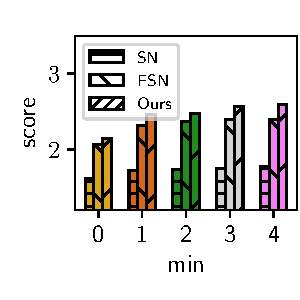
\includegraphics[width=1\textwidth]{chapters/vibvoice/figure/noise_enrollment_0.pdf}
        %\vspace{-1.99em}
        \caption{PESQ.}
        \label{fig:vibvoice_noise_duration_0}
        \end{subfigure}
    \begin{subfigure}{0.32\columnwidth}
        \centering
        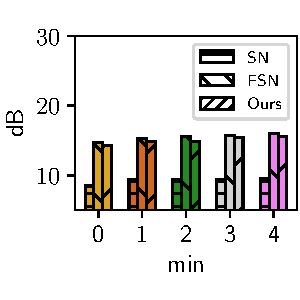
\includegraphics[width=1\textwidth]{chapters/vibvoice/figure/noise_enrollment_1.pdf}
        %\vspace{-1.99em}
        \caption{SNR.}
        \label{fig:vibvoice_noise_duration_1}
         \end{subfigure}
    \begin{subfigure}{0.32\columnwidth}
        \centering
        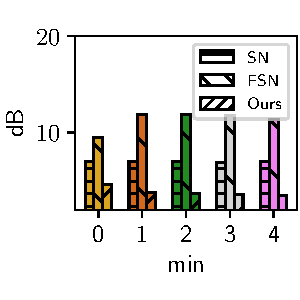
\includegraphics[width=1\textwidth]{chapters/vibvoice/figure/noise_enrollment_2.pdf}
        %\vspace{-1.99em}
        \caption{LSD.}
        \label{fig:vibvoice_noise_duration_2}
         \end{subfigure}
    %\vspace{-1em}
    \caption{Impact of calibration time.}
    \label{fig:vibvoice_noise_duration}
    %\vspace{-1em}
\end{figure}

\begin{figure}
     %\vspace{-0.5em}
    \begin{subfigure}{0.32\columnwidth}
        \centering
        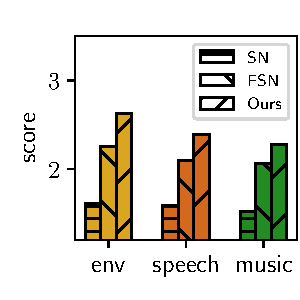
\includegraphics[width=1\textwidth]{chapters/vibvoice/figure/noise_type_0.pdf}
        %\vspace{-1.99em}
        \caption{PESQ.}
        \label{fig:vibvoice_noise_type_0}
        \end{subfigure}
    \begin{subfigure}{0.32\columnwidth}
        \centering
        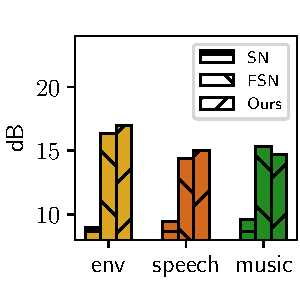
\includegraphics[width=1\textwidth]{chapters/vibvoice/figure/noise_type_1.pdf}
        %\vspace{-1.99em}
        \caption{SNR.}
        \label{fig:vibvoice_noise_type_1}
         \end{subfigure}
    \begin{subfigure}{0.32\columnwidth}
        \centering
        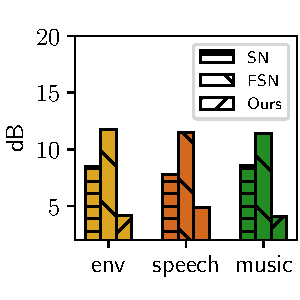
\includegraphics[width=1\textwidth]{chapters/vibvoice/figure/noise_type_2.pdf}
        %\vspace{-1.99em}
        \caption{LSD.}
        \label{fig:vibvoice_noise_type_2}
         \end{subfigure}
    %\vspace{-1em}
    \caption{Impact of noise types.}
    \label{fig:vibvoice_noise_type}
    %\vspace{-1em}
\end{figure}

\begin{figure}
    %\vspace{-0.5em}
    \begin{subfigure}{0.32\columnwidth}
        \centering
        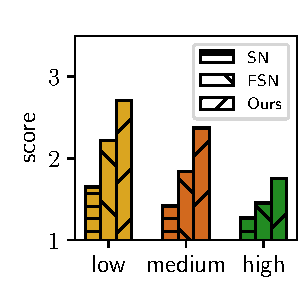
\includegraphics[width=1\textwidth]{chapters/vibvoice/figure/noise_level_0.pdf}
        %\vspace{-1.99em}
        \caption{PESQ.}
        \label{fig:vibvoice_noise_level_0}
        \end{subfigure}
    \begin{subfigure}{0.32\columnwidth}
        \centering
        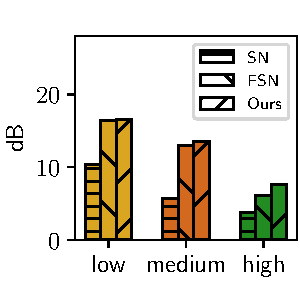
\includegraphics[width=1\textwidth]{chapters/vibvoice/figure/noise_level_1.pdf}
        %\vspace{-1.99em}
        \caption{SNR.}
        \label{fig:vibvoice_noise_level_1}
         \end{subfigure}
    \begin{subfigure}{0.32\columnwidth}
        \centering
        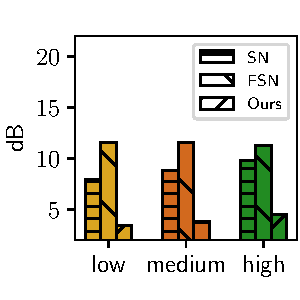
\includegraphics[width=1\textwidth]{chapters/vibvoice/figure/noise_level_2.pdf}
        %\vspace{-1.99em}
        \caption{LSD.}
        \label{fig:vibvoice_noise_level_2}
         \end{subfigure}
    %\vspace{-1em}
    \caption{Impact of noise levels.}
    \label{fig:vibvoice_noise_level}
    %\vspace{-1em}
\end{figure}

\begin{figure}
%\vspace{-0.5em}
    \begin{subfigure}{0.32\columnwidth}
        \centering
        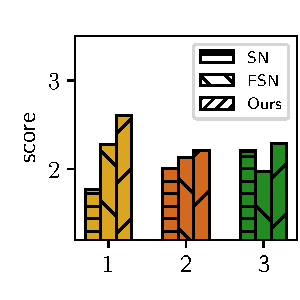
\includegraphics[width=1\textwidth]{chapters/vibvoice/figure/noise_number_0.pdf}
        %\vspace{-1.99em}
        \caption{PESQ.}
        \label{fig:vibvoice_noise_number_0}
        \end{subfigure}
        \hfill
    \begin{subfigure}{0.32\columnwidth}
        \centering
        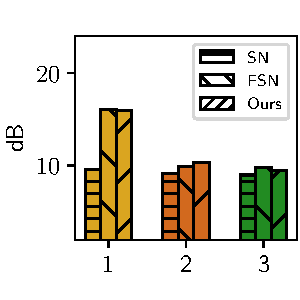
\includegraphics[width=1\textwidth]{chapters/vibvoice/figure/noise_number_1.pdf}
        %\vspace{-1.99em}
        \caption{SNR.}
        \label{fig:vibvoice_noise_number_1}
         \end{subfigure}
          \hfill
    \begin{subfigure}{0.32\columnwidth}
        \centering
        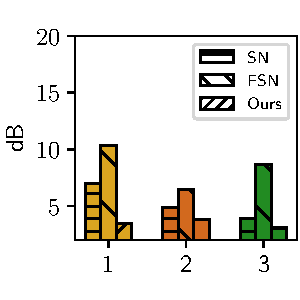
\includegraphics[width=1\textwidth]{chapters/vibvoice/figure/noise_number_2.pdf}
        %\vspace{-1.99em}
        \caption{LSD.}
        \label{fig:vibvoice_noise_number_2}
         \end{subfigure}
    %\vspace{-1em}
    \caption{Number of noise sources.}
    %\vspace{-1em}
    \label{fig:vibvoice_noise_number}
    % %\vspace{-1em}
\end{figure}




\begin{figure}
    \begin{subfigure}{0.3\columnwidth}
        \centering
        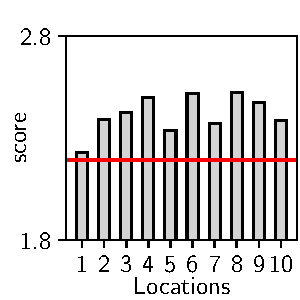
\includegraphics[width=1\textwidth]{chapters/vibvoice/figure/locations_0.pdf}
        %\vspace{-1em}
        \caption{PESQ.}
        \label{fig:vibvoice_location_0}
        \end{subfigure}
    \begin{subfigure}{0.3\columnwidth}
        \centering
        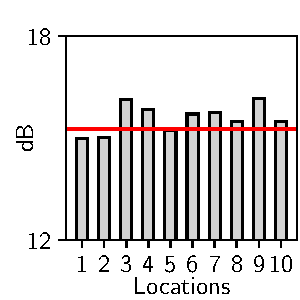
\includegraphics[width=1\textwidth]{chapters/vibvoice/figure/locations_1.pdf}
        %\vspace{-1em}
        \caption{SNR.}
        \label{fig:vibvoice_location_1}
         \end{subfigure}
    \begin{subfigure}{0.3\columnwidth}
        \centering
        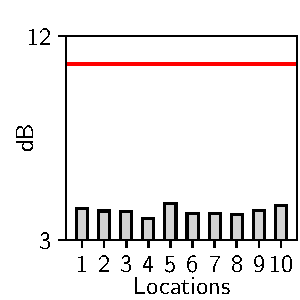
\includegraphics[width=1\textwidth]{chapters/vibvoice/figure/locations_2.pdf}
        %\vspace{-1em}
        \caption{LSD.}
        \label{fig:vibvoice_location_2}
         \end{subfigure}
    %\vspace{-1em}
    \caption{VibVoice on different head locations. Red line: the performance of the baseline, i.e., FullSubNet.}
    \label{fig:vibvoice_locations}
    %\vspace{-1em}
\end{figure}


\begin{figure}
    \begin{subfigure}{0.3\columnwidth}
        \centering
        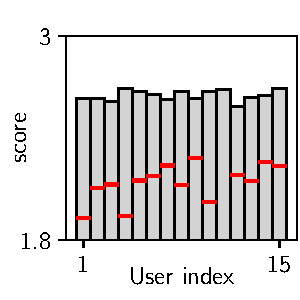
\includegraphics[width=1\textwidth]{chapters/vibvoice/figure/per_user_0.pdf}
        %\vspace{-1em}
        \caption{PESQ.}
        \label{fig:vibvoice_per_user_0}
        \end{subfigure}
    \begin{subfigure}{0.3\columnwidth}
        \centering
        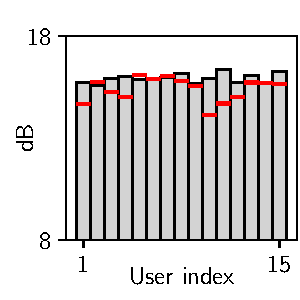
\includegraphics[width=1\textwidth]{chapters/vibvoice/figure/per_user_1.pdf}
        %\vspace{-1em}
        \caption{SNR.}
        \label{fig:vibvoice_per_user_1}
        \end{subfigure}
    \begin{subfigure}{0.3\columnwidth}
        \centering
        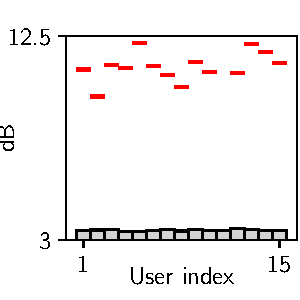
\includegraphics[width=1\textwidth]{chapters/vibvoice/figure/per_user_2.pdf}
        %\vspace{-1em}
        \caption{LSD.}
        \label{fig:vibvoice_per_user_2}
         \end{subfigure}
    %\vspace{-1em}
    \caption{VibVoice on different users. Red line: the performance of the baseline, i.e., FullSubNet.}
    \label{fig:vibvoice_per_user}
    %\vspace{-1em}
\end{figure}



\begin{figure}
% %\vspace{-1em}
    \begin{subfigure}{0.32\columnwidth}
        \centering
        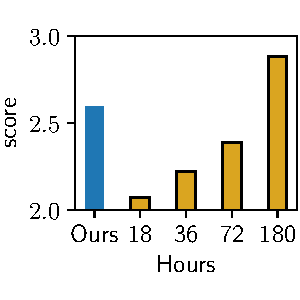
\includegraphics[width=1\textwidth]{chapters/vibvoice/figure/data_augmentation_0.pdf}
        %\vspace{-1.99em}
        \caption{PESQ.}
        \label{fig:vibvoice_data_augmentation_0}
        \end{subfigure}
    \begin{subfigure}{0.32\columnwidth}
        \centering
        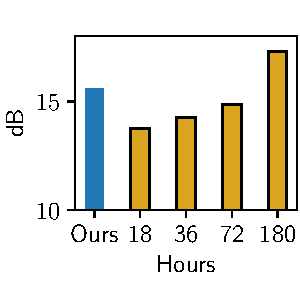
\includegraphics[width=1\textwidth]{chapters/vibvoice/figure/data_augmentation_1.pdf}
        %\vspace{-1.99em}
        \caption{SNR.}
        \label{fig:vibvoice_data_augmentation_1}
         \end{subfigure}
    \begin{subfigure}{0.32\columnwidth}
        \centering
        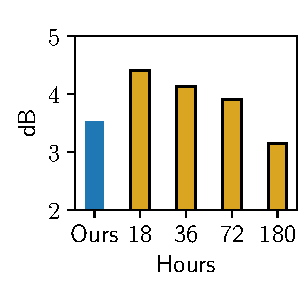
\includegraphics[width=1\textwidth]{chapters/vibvoice/figure/data_augmentation_2.pdf}
        %\vspace{-1.99em}
        \caption{LSD.}
        \label{fig:vibvoice_data_augmentation_2}
         \end{subfigure}
    %\vspace{-1em}
    \caption{Effectiveness of data augmentation. Blue bars: VibVoice using less than three-hour paired data with augmentation. Yellow bars: VibVoice using 18- to 180-hour paired data without augmentation.}
    \label{fig:vibvoice_data_augmentation}
\end{figure}

\begin{table}
\centering
\begin{tabular}{cccc}\toprule
& PESQ&SNR&LSD \\ \midrule
VibVoice              & 2.6 & 15.6 & 3.5  \\ 
w/o auxiliary decoder & 2.5 & 15.1 & 4.4 \\ 
w/o augmentation      & 1.9 & 14   & 5\\ 
w/o Gaussian approx   & 2.4 & 15.2 & 4.2 \\ 
Accelerometer sample rate: 1200 Hz & 2.47 & 14.4 & 4.2 \\ 
Accelerometer sample rate: 800 Hz & 2.45 & 14.3 & 4.5 \\ 
Accelerometer sample rate: 400 Hz & 2.4 & 14.2 & 4.4 \\ \bottomrule
\end{tabular}
\caption{\label{table3}Ablation study.}
\end{table}

\subsection{Ablation Study}
We conduct an ablation study to understand the performance of different design components in VibVoice. The performance of VibVoice without different components is listed in Table \ref{table3}.

\noindent\textbf{No auxiliary decoder}. First, we remove the self-supervise loss, meaning the audio may dominate the model. The results indicate that the variant slightly degrades by 0.1 in PESQ, 0.3 in SNR, and 0.8 in LSD, respectively.

\noindent\textbf{No data augmentation}.
Second, we remove the data augmentation based on Bone Conduction Function. The performance significantly degrades to 1.9 in PESQ, 14 in SNR, and 5 in LSD. According to the definition of ITU and mean opinion score (MOS), the audio quality is poor when the score drops from 2.5 to 1.9 \citep{Perceptu66:online}. This result aligns with our motivation that a small-scale self-collected dataset is insufficient to train a strong neural network.

\noindent\textbf{No Gaussian approximation}.
Third, the Bone Conduction Function is modeled by only the mean, while the variance is zero. The performance drops 0.2 in PESQ, 0.4 in SNR, and 0.5 for LSD, indicating that our Gaussian approximation is close to the nature of the Bone Conduction Function.

\noindent\textbf{Lower sample rate}.
The frequency response in Fig. \ref{fig:vibvoice_bcf} shows that the speech information from above 600 Hz is very limited. Hence, we evaluate the performance of VibVoice with a lower sample rate by downsampling the acceleration data to 1200 Hz, 800 Hz, and 400 Hz. The results show that VibVoice is robust to various sample rates, which consume less power in processing and communication. When the sample rate is 800 Hz, the output's PESQ only degrades $10\%$.

\subsection{On-Site Evaluation}
In the following, we conduct extensive experiments to validate the performance of VibVoice with ongoing noise in the wild. The volunteers are asked to read the same content as the experiments in Section. \ref{sec:vibvoice_overall_eval}. Apart from the environmental noises, we use a smartphone (i.e., Huawei P30) to play recorded speech and ask a volunteer to speak one meter away as the interference. The speech content of the competing speaker is irrelevant to the target speech. We collect 10 minutes of data with about 3dB SNR at each test location.
Unlike synthetic noisy speech, we can neither capture the ground truth of clean speech and evaluate the metrics like SNR and PESQ nor train the model. Instead, we use the result of Automatic Speech Recognition \citep{ravanelli2021speechbrain} to evaluate the quality of the speech. We use Word Error Rate ($\text{WER}=\frac{S+D+I}{N}$) as the evaluation metric, where S is the number of substitutions, D is the number of deletions, I is the number of insertions, and N is the number of words in the reference. The higher the value of WER, the lower the audio quality.
To better evaluate the performance of VibVoice, we further define the relative improvement of WER in percentage as $\frac{(WER_{o} -  WER_{v})}{WER_{o}}\times100 \%$, where $WER_{o}$ refers to the WER of the original audio, $WER_{v}$ refers to the WER of VibVoice.

\begin{figure}[t]
    \centering
    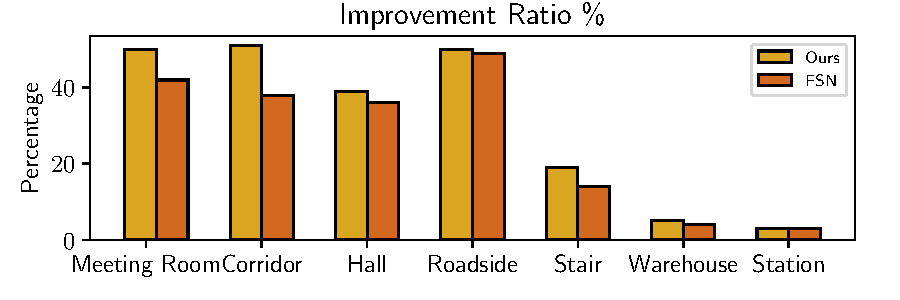
\includegraphics[width=\columnwidth]{chapters/vibvoice/figure/environments.pdf}
    %\vspace{-1em}
    \caption{Different environments.}
    %\vspace{-1em}
    \label{fig:vibvoice_environment}
\end{figure}

\subsubsection{\textbf{Environments}}
We evaluate VibVoice in diverse indoor and outdoor environments, including the meeting room, corridor, stairs, lumber room, and railway station. 
We note that the experiment conducted in the real world naturally contains diverse environmental noises (e.g., train, car, construction, wind) and competing speakers. The results in Fig. \ref{fig:vibvoice_environment} show that VibVoice effectively improves speech quality in most environments.
Most existing works have good performance in statistical noises like machinery noises, however, they perform badly when there are competing speakers in the same room, which is a common indoor scenario of voice communication.
 Although speech enhancement is challenging in small spaces like a meeting room and corridor due to the strong multi-path effect, VibVoice can still improve the speech quality and achieve an improvement ratio of over 50\%, and 48\%, respectively. VibVoice also achieves a 37$\%$ improvement for the hall, 29$\%$ for the outdoor square, and 19\% in the scene of the outdoor stair when there is intermittent construction noise. We note that in both the warehouse and station, the improvement of VibVoice is marginal. This is mainly because that AirPods already perform well in these scenarios. In comparison, VibVoice keeps outperforming FSN with much less latency. 

\subsubsection{\textbf{Earphones}}
We deploy VibVoice on three popular TWS earphones, i.e., Apple AirPods Pro, Huawei FreeBuds Pro, and Samsung GalaxyBuds Pro. During the experiment, we turn on all available acoustic signal processing algorithms provided by the manufacturers, including speech enhancement and noise suppression.
The results show that the WER with a competing speaker is $60\%$ for AirPods, $66\%$ for FreeBuds, and $160\%$ for GalaxyBuds, respectively. Due to the different designs of the earphones, we do not implement VibVoice on other earphones. Since VibVoice can effectively reduce the WER of AirPods Pro by $50\%$, we envision that VibVoice can be extended to other earphones.

\subsubsection{\textbf{User movements}}
We further evaluate the performance of VibVoice when the user is moving. We ask volunteers to move in the room with a speed of around $1\,\text{m/s}$.  
The result shows the improvement for a still volunteer is 58.3 $\%$, while the same moving volunteer is 57.1$\%$.
The standard deviation for the still and moving case is 29.9 $\%$ and 30.4$\%$, respectively. Although the improvement ratio slightly drops, VibVoice still preserves its performance under regular movements. 

\begin{table}
\centering
%\vspace{-1em}
\begin{tabular}{cccc}\toprule
& VibVoice & FSN & SN \\ \midrule
Desktop CPU    & 0.05 &0.27  & 0.5 \\ 
Desktop GPU    & 0.016&0.034 & 0.07\\ 
P30    & 0.16 &5     & 1.9 \\ 
Mate20 & 0.29 &4.6   & 1.7\\ 
Pixel7 & 0.31 &5.2   & 1.4\\ \bottomrule
\end{tabular}
\caption{\label{table4}Runtime analysis (second/instance).}
%\vspace{-1em}
\end{table}

\subsection{Runtime Evaluation}
\label{sec:vibvoice_runtime}
We test the execution latency of VibVoice and the two baselines (i.e., FSN \citep{hao2021fullsubnet} and SN \citep{tagliasacchi2020seanet}) on a desktop PC (i.e., i7-11700k CPU and RTX 3060 GPU) and three smartphones (i.e., Huawei P30, Huawei Mate20, and Google Pixel 7). We run the inference of 5 seconds clip 100 times and record the mean latency. 
The results in Table \ref{table4} show that VibVoice reduces up to $31\times$ and $12\times$ less latency on average than FSN and SN, respectively. On the other hand, the results show that VibVoice exhibits a greater advantage in runtime for low-end devices.
In conclusion, VibVoice can support real-time voice applications with a delay of fewer than 0.6 seconds (i.e., two times the inference latency) for processing 5 seconds audio clip. The real-time factor is only 0.12, significantly less than the minimal requirement, which means less energy consumption and space to process other tasks.

\section{User Study}
\label{sec:vibvoice_user-study}
We recruit 35 volunteers to study the real perceived experience of VibVoice.

%\vspace{0.5em}
\noindent\textbf{Questionnaire Design}.
We play a few recordings from the dataset described in Section 5.1 to volunteers. The length of each sentence is clipped or padded to 5 seconds.
The first part is to evaluate the intelligibility of reconstructed speech. The participants are asked to listen to the audio clips enhanced by VibVoice and write down the sentences. We use WER to evaluate the results.
In the second part of the study, participants listen to two audio clips with the same content and choose the audio with better quality in their perception. This study evaluates whether the reconstructed speech improves the user experience or not.
We conduct two kinds of comparisons five times. One type is to ask participants to choose between audio enhanced by VibVoice and the original noisy audio. The second kind is to ask participants to choose between audio enhanced by VibVoice and the baseline (i.e., FSN). We use the correct ratio $\frac{P}{P+N}$ to represent the improvement of VibVoice, in which $P$ and $N$ are the numbers of choosing VibVoice and negative vice versa.


\subsection{Study Result}
In the first part, VibVoice achieves an overall WER of $21.5\%$, which supports intelligibility of the reconstructed speech.
For perceived quality, $87\%$ of the participants choose VibVoice over the baseline, and $72\%$ choose VibVoice over the original noisy audio.
We also asked participants why they sometimes preferred the original audio over the baseline. The baseline can produce acoustic artifacts and suppress the target speaker. Some participants observed that repeated listening reduced the effect of artifacts and suppression, but the baseline speech still caused misunderstandings for first-time listeners. Overall, the user study shows that VibVoice improves perceived speech quality compared with both the original audio and the baseline.
